\documentclass[12 pt]{article}
\usepackage[utf8]{inputenc}
\usepackage[T1]{fontenc}
\usepackage{amsmath}
\usepackage{amsfonts}
\usepackage{amssymb}
\usepackage[version=4]{mhchem}
\usepackage{stmaryrd}
\usepackage{graphicx}

\usepackage{listings} % Required for insertion of code
\usepackage{xcolor} % Required for custom colors

% Define custom colors
\definecolor{codegreen}{rgb}{0,0.6,0}
\definecolor{codegray}{rgb}{0.5,0.5,0.5}
\definecolor{codepurple}{rgb}{0.58,0,0.82}
\definecolor{backcolour}{rgb}{0.95,0.95,0.92}

% Setup the style for code listings
\lstdefinestyle{mystyle}{
    backgroundcolor=\color{backcolour},   
    commentstyle=\color{codegreen},
    keywordstyle=\color{magenta},
    numberstyle=\tiny\color{codegray},
    stringstyle=\color{codepurple},
    basicstyle=\ttfamily\footnotesize,
    breakatwhitespace=false,         
    breaklines=true,                 
    captionpos=b,                    
    keepspaces=true,                 
    numbers=left,                    
    numbersep=5pt,                  
    showspaces=false,                
    showstringspaces=false,
    showtabs=false,                  
    tabsize=2
}

% Activate the style
\lstset{style=mystyle}

\graphicspath{ {./images/} }

\title{Ch14 Spring 2024 \\
 Problem set 1 \\
 due April 11, 2024 }

\author{}
\date{}


\begin{document}
\maketitle
unless otherwise stated, assume $\mathrm{T}=25^{\circ} \mathrm{C}$ and that activities = concentrations.

unless otherwise specified, give answers to 3 significant figures.

\section{}
\begin{enumerate}
  \item (30 pts total) At $25^{\circ} \mathrm{C}$ and 1 atm, the standard free energies $\left(\mathrm{G}^{\circ}{ }_{\mathrm{f}}\right)$ of formation of benzene in the liquid and gas phase have the following values:
\end{enumerate}

\begin{center}
\begin{tabular}{|c|c|}
\hline
phase & $\mathrm{G}^{\circ}{ }_{\mathrm{f}}\left(\mathrm{kJ} \mathrm{mol}^{-1}\right)$ \\
\hline
liquid & 124.5 \\
\hline
gas & 129.7 \\
\hline
\end{tabular}
\end{center}

\subsection{}
1a. (10 pts) Which phase (liquid or gas) is more stable under these conditions? Explain briefly (12 sentences)\\
The liquid phase, because it has the lower free energy of formation.

\subsection{}
1b. (10 pts) Calculate the vapor pressure of benzene under these conditions. Express your answer in both $\mathrm{Pa}$ and $\mathrm{mm} \mathrm{Hg}$. $(1 \mathrm{~atm}=101325 \mathrm{~Pa}=760 \mathrm{~mm} \mathrm{Hg}$ )\\
We can use the formula:
\begin{equation}
  \Delta G = -RT \ln P
\end{equation}
to find the vapor pressure of benzene. We can rearrange the formula to solve for $P$:
\begin{equation}
  P = e^{-\frac{\Delta G}{RT}}
\end{equation}
The change in free energy is given by:
\begin{equation}
  \Delta G = G_{\text{gas}} - G_{\text{liquid}} = 129.7 - 124.5 = 5.2 \text{ kJ/mol} = 5.2 \times 10^3 \text{ J/mol}
\end{equation}
Substituting the values into the formula, we get:
\begin{equation}
  P_\text{atm} = 0.123 \text{ atm} = 12400 \text{ Pa} = 93.2 \text{ mm Hg}
\end{equation}
% Inline Python code in the document
\begin{lstlisting}[language=Python]
import math

# Constants
delta_G = 5.2 * 1000  # Change in free energy, in J/mol
R = 8.314  # Universal gas constant, in J/(molxK)
T = 298  # Temperature, in K

# Calculating vapor pressure in atm
P_atm = math.exp(-delta_G / (R * T))

# Conversion factors
Pa_per_atm = 101325  # Pascal per atm
mmHg_per_atm = 760  # mm Hg per atm

# Converting to Pa and mm Hg
P_Pa = P_atm * Pa_per_atm
P_mmHg = P_atm * mmHg_per_atm

P_atm, P_Pa, P_mmHg

\end{lstlisting}
\subsection{}
1c. (10 pts) If $10 \mathrm{mls}$ of liquid benzene are placed in an evacuated 1 liter flask, how much benzene (in milliliters) will evaporate to reach equilibrium at $25^{\circ} \mathrm{C}$ ? i.e. - how many mls of liquid benzene must evaporate to achieve the vapor pressure calculated in problem $1 \mathrm{~b}$ ? If you are unsure of your answer to $1 \mathrm{~b}$, use $\mathrm{P}=100 \mathrm{~mm} \mathrm{Hg}$ (accurate to within 10\%)

Other potentially useful information: the molecular weight of benzene is $78.11 \mathrm{gm} \mathrm{mol}^{-1}$ and the density is $0.876 \mathrm{gm} \mathrm{ml}^{-1}\left(876 \mathrm{~kg} \mathrm{~m}^{-3}\right)$. Assume ideal gas behavior; values for the gas constant $\mathrm{R}$ are $8.3144 \mathrm{~J} \mathrm{~mol}^{-1} \mathrm{~K}^{-1}$ and 0.08206 liter atm $\mathrm{mol}^{-1} \mathrm{~K}^{-1}$, in $\mathrm{SI}$ and non-SI units, respectively. You may neglect the volume of the liquid in working this problem (ie - you may assume that the volume of the gas phase is $1 \mathrm{~L}$ ).\\
Our algorithm to solve this problem is as follows:
\begin{enumerate}
  \item Calculate the number of moles of benzene in the gas phase at equilibrium.
  \item Calculate the mass of evaporated benzene.
  \item Calculate the volume of benzene that evaporated.
\end{enumerate}
I chose to use the value of $100 \text{ mm Hg}$ for the vapor pressure in this calculation.
To achieve the vapor pressure given in the instructions, $0.480 \text{ mL}$ of liquid benzene must evaporate.
% Inline Python code in the document
\begin{lstlisting}[language=Python]
# Given data
P_mmHg = 100  # Vapor pressure in mm Hg
P_atm = P_mmHg / 760  # Converting pressure to atm
V_L = 1  # Volume in liters
R_L_atm_per_mol_K = 0.08206  # Gas constant in liter atm per mol K
T_C = 25  # Temperature in Celsius
T_K = T_C + 273.15  # Converting temperature to Kelvin

# Calculating moles of benzene vapor at equilibrium using the ideal gas law
n_moles = (P_atm * V_L) / (R_L_atm_per_mol_K * T_K)

# Given molecular weight and density of benzene
molecular_weight_benzene = 78.11  # g/mol
density_benzene_g_per_ml = 0.876  # g/ml

# Calculating mass of evaporated benzene
mass_evaporated_g = n_moles * molecular_weight_benzene

# Calculating volume of evaporated benzene in ml
volume_evaporated_ml = mass_evaporated_g / density_benzene_g_per_ml

n_moles, mass_evaporated_g, volume_evaporated_ml

\end{lstlisting}
\section{}
\begin{enumerate}
  \setcounter{enumi}{1}
  \item (40 pts total) The hydrolysis of adenosine triphosphate (ATP) to form ADP + inorganic phosphate $(\mathrm{Pi}): A T P \rightarrow A D P+P_{i}$, is an important reaction in bioenergetics. Under standard conditions $25^{\circ} \mathrm{C}$ and $1 \mathrm{~atm}, \Delta \mathrm{G}^{\circ}=-30 \mathrm{~kJ} \mathrm{~mol}^{-1}$.
\end{enumerate}

\subsection{}
2a. (10 pts) What is $K_{\text {eq }}$ for this reaction?\\
We can use the formula:
\begin{equation}
  \Delta G = -RT \ln K_{\text{eq}}
\end{equation}
to find the equilibrium constant for the reaction. We can rearrange the formula to solve for $K_{\text{eq}}$:
\begin{equation}
  K_{\text{eq}} = e^{-\frac{\Delta G}{RT}}
\end{equation}
Substituting the values into the formula, we get:
\begin{equation}
  K_{\text{eq}} = 1.80 \times 10^{5}
\end{equation}
% Inline Python code in the document
\begin{lstlisting}[language=Python]
# Given data
delta_G_kJ_per_mol = -30  # Change in free energy, in kJ/mol
delta_G_J_per_mol = delta_G_kJ_per_mol * 1000  # Convert kJ/mol to J/mol
R = 8.314  # Universal gas constant, in J/(molxK)
T_C = 25  # Temperature in Celsius
T_K = T_C + 273.15  # Converting temperature to Kelvin

# Calculating Keq
K_eq = math.exp(-delta_G_J_per_mol / (R * T_K))

K_eq

\end{lstlisting}

\subsection{}
2b. (10 pts) Under physiological conditions, the concentration of ADP is kept to very low values in the cell by continual rephosphorylation to form ATP. What is $\Delta \mathrm{G}$ under physiological conditions, when $(A T P)=10 \mathrm{mM},(\mathrm{ADP})=10 \mu \mathrm{M}$ and $(\mathrm{Pi})=10 \mathrm{mM}$ ?\\
In order to solve this problem, we want to consider the relationship:
\begin{equation}
  \Delta G = \Delta G^\circ + RT \ln Q
\end{equation}
where $\Delta G$ is the change in free energy, $\Delta G^\circ$ is the standard change in free energy, $R$ is the universal gas constant, $T$ is the temperature, and $Q$ is the reaction quotient. The reaction quotient is given by:
\begin{equation}
  Q = \frac{[\text{ADP}] [\text{Pi}]}{[\text{ATP}]}
\end{equation}
Performing this computation, we get:
\begin{equation}
  \Delta G = -58.5 \text{ kJ/mol}
\end{equation}
% Inline Python code in the document
\begin{lstlisting}[language=Python]
# Given data
delta_G_zero_J_per_mol = -30000  # Standard free energy change in J/mol
ATP_concentration_mM = 10  # mM
ADP_concentration_uM = 10  # uM
Pi_concentration_mM = 10  # mM

# Convert concentrations to M (mol/L)
ATP_concentration_M = ATP_concentration_mM * 10**-3
ADP_concentration_M = ADP_concentration_uM * 10**-6
Pi_concentration_M = Pi_concentration_mM * 10**-3

# Calculate Q
Q = (ADP_concentration_M * Pi_concentration_M) / ATP_concentration_M

# Calculate Delta G under physiological conditions
Delta_G = delta_G_zero_J_per_mol + (R * T_K * math.log(Q))

Delta_G

\end{lstlisting}
\subsection{}
2c. $(10$ pts) Starting with $(A T P)=0 \mathrm{mM},(A D P)=1 \mathrm{mM},(\mathrm{Pi})=1 \mathrm{mM}$, what is the concentration of ATP at equilibrium?\\
Previously, we calculated the equilibrium constant for the reaction as $1.80 \times 10^{5}$. We can use this value to calculate the concentration of ATP at equilibrium. The reaction quotient $Q$ is given by:
\begin{equation}
  Q = \frac{[\text{ADP}] [\text{Pi}]}{[\text{ATP}]}
\end{equation}
At equilibrium, $Q = K_{\text{eq}}$. We can rearrange the formula to solve for $[\text{ATP}]$:
\begin{equation}
  [\text{ATP}] = \frac{[\text{ADP}] [\text{Pi}]}{K_{\text{eq}}}
\end{equation}
Substituting the values into the formula, we get:
\begin{equation}
\boxed{[\text{ATP}] = 5.55 \times 10^{-12} \text{ M}}
\end{equation}
% Inline Python code in the document
\begin{lstlisting}[language=Python]
# Recalculating ATP concentration at equilibrium
ADP_concentration_M = 1e-3  # M
Pi_concentration_M = 1e-3  # M

# Calculating ATP concentration at equilibrium using the corrected formula
ATP_concentration_at_equilibrium_M = (ADP_concentration_M * Pi_concentration_M) / K_eq_value

ATP_concentration_at_equilibrium_M

\end{lstlisting}
\subsection{}
2d. $(10$ pts) Starting with $(A T P)=0 \mathrm{mM},(A D P)=1 \mathrm{mM},(\mathrm{Pi})=1000 \mathrm{mM}$, what is the concentration of ATP at equilibrium?

Note: the equilibrium for ATP hydrolysis greatly favors the products ADP and Pi, so that the final product concentrations ((ADP) and (Pi)) may be equated to the initial product concentrations for problems $2 \mathrm{c}$ and $2 \mathrm{~d}$.\\
Using the similar procedure as was done previously:
\begin{equation}
\boxed{[\text{ATP}] = 5.55 \times 10^{-9} \text{ M}}
\end{equation}
% Inline Python code in the document
\begin{lstlisting}[language=Python]
# Updated initial conditions for problem 2d
Pi_concentration_M_updated = 1000e-3  # M, converting from mM to M

# Recalculating ATP concentration at equilibrium with updated Pi concentration
ATP_concentration_at_equilibrium_M_updated = (ADP_concentration_M * Pi_concentration_M_updated) / K_eq_value

ATP_concentration_at_equilibrium_M_updated

\end{lstlisting}
\section{}
\begin{enumerate}
  \setcounter{enumi}{2}
  \item (10 pts) The following reaction has an equilibrium constant $\mathrm{K}=10$ at $25{ }^{\circ} \mathrm{C}$ (when concentrations are defined using the Molar (moles/liter) solution convention)
\end{enumerate}

$$
A+B \stackrel{K}{\rightleftharpoons} C
$$

What are the concentrations of $(A),(B)$ and $(C)$ at equilibrium, starting with $(A)=(B)=0.0 \mathrm{M}$ and (C) $=0.1 \mathrm{M}$ ? \\
The equilibrium constant is given by:
\begin{equation}
  K = \frac{[C]}{[A][B]}
\end{equation}
and we also have mass balance, so:
\begin{equation}
  [A] = [B] =x \quad \text{and} \quad [C] = 0.1 - x
\end{equation}
Using this information, we find:
\begin{equation}
\boxed{[A] = [B] = 0.062 \text{ M}, \quad [C] = 0.038 \text{ M}}
\end{equation}
% Inline Python code in the document
\begin{lstlisting}[language=Python]
from sympy import symbols, Eq, solve

# Define symbol
x = symbols('x')

# Given data
K = 10  # Equilibrium constant
initial_C = 0.1  # Initial concentration of C in M

# Equilibrium expressions
# [C] = initial_C - x, [A] = x, [B] = x

# Equilibrium constant expression
equation = Eq(K, (initial_C - x) / (x**2))

# Solve for x
x_solution = solve(equation, x)

# Filter out the negative solution since concentration cannot be negative
x_equilibrium = [sol for sol in x_solution if sol > 0]

# Calculate equilibrium concentrations
A_eq = B_eq = x_equilibrium[0]
C_eq = initial_C - x_equilibrium[0]

A_eq, B_eq, C_eq

\end{lstlisting}
\section{}
\begin{enumerate}
  \setcounter{enumi}{3}
  \item (10 pts) The following reaction has an equilibrium constant $\mathrm{K}=10$ at $25{ }^{\circ} \mathrm{C}$ (when concentrations are defined using the Molar (moles/liter) solution convention)
\end{enumerate}

$$
2 A \stackrel{K}{\rightleftharpoons} C
$$

What are the concentrations of $(A)$ and $(C)$ at equilibrium, starting with $(A)=0.0 \mathrm{M}$ and $(C)=0.1$ $\mathrm{M}$ ?\\
Because the stoichiometry of the reaction is different, the expression for the equilibrium constant is:
\begin{equation}
  K = \frac{[C]}{[A]^2}
\end{equation}
and we also have mass balance, so:
\begin{equation}
  [C] = 0.1 - x, \quad [A] = 2x
\end{equation}
Using this information, we find:
\begin{equation}
\boxed{[A] = 0.078 \text{ M}, \quad [C] = 0.061 \text{ M}}
\end{equation}
% Inline Python code in the document
\begin{lstlisting}[language=Python]
# Define a new symbol for x representing the change for this reaction
x_2A_to_C = symbols('x')

# Given data for the new problem
K_2A_to_C = 10  # Equilibrium constant
initial_C_2A_to_C = 0.1  # Initial concentration of C in M

# Equilibrium expressions for the reaction 2A <-> C
# [C] = initial_C - x, [A] = 2x

# Equilibrium constant expression for 2A <-> C
equation_2A_to_C = Eq(K_2A_to_C, (initial_C_2A_to_C - x_2A_to_C) / (2*x_2A_to_C)**2)

# Solve for x for the 2A <-> C reaction
x_solution_2A_to_C = solve(equation_2A_to_C, x_2A_to_C)

# Filter out the negative solution since concentration cannot be negative
x_equilibrium_2A_to_C = [sol for sol in x_solution_2A_to_C if sol > 0]

# Calculate equilibrium concentrations for A and C
A_eq_2A_to_C = 2 * x_equilibrium_2A_to_C[0]
C_eq_2A_to_C = initial_C_2A_to_C - x_equilibrium_2A_to_C[0]

A_eq_2A_to_C, C_eq_2A_to_C

\end{lstlisting}

\section{}
\begin{enumerate}
  \setcounter{enumi}{4}
  \item (10 pts) Acetic acid in the vapor phase exists as an equilibrium between monomeric and dimeric forms:
\end{enumerate}

\begin{figure}[h]
  \centering
  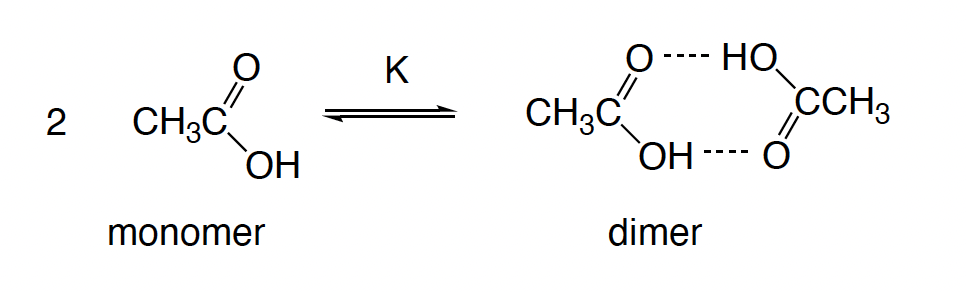
\includegraphics[width=0.5\textwidth]{image.png}
  \caption{Acetic acid equilibrium}
\end{figure}

At $\mathrm{T}=400 \mathrm{~K}$ and a total pressure $\mathrm{P}=1 \mathrm{~atm}$, the monomer - dimer equilibrium constant $\mathrm{K}=2.02$ (defined when the gas pressures are measured in atm). Calculate partial pressures (in atm) of the monomeric and dimeric species under these conditions.\\
At equilibrium:
\begin{equation}
  P_{\text{monomer}} + P_{\text{dimer}} = P_{\text{total}}
\end{equation}
The equilibrium constant is given by:
\begin{equation}
  K = \frac{P_{\text{dimer}}}{P_{\text{monomer}}^2}
\end{equation}
Performing some algebra with these equations, we get:
\begin{equation}
  P_{\text{monomer}} = 0.498 \text{ atm}, \quad P_{\text{dimer}} = 0.502 \text{ atm}
\end{equation}
% Inline Python code in the document
\begin{lstlisting}[language=Python]
# Define symbol for x, representing the partial pressure of the monomer
x = symbols('x', real=True, positive=True)

# Given data
K_value = 2.02  # Equilibrium constant
total_pressure = 1  # Total pressure in atm

# Equilibrium expressions
# For monomer (A), P_monomer = x
# For dimer (A2), P_dimer = total_pressure - x

# Equilibrium constant expression K = P_dimer / P_monomer^2
equation = Eq(K_value, (total_pressure - x) / x**2)

# Solve for x (P_monomer)
x_solution = solve(equation, x)

# Filter out the negative and non-real solutions since pressure cannot be negative or non-real
x_real_solutions = [sol.evalf() for sol in x_solution if sol.is_real and sol > 0]

# Select the first solution (there should only be one positive real solution in this physical context)
P_monomer_atm = x_real_solutions[0]

# Calculate P_dimer using the total pressure and the calculated P_monomer
P_dimer_atm = total_pressure - P_monomer_atm

P_monomer_atm, P_dimer_atm

\end{lstlisting}


\end{document}